\section{Die分区(Chiplet划分)}

首先是名词解析,“Die”(中文常译为“晶粒”或“裸芯”)是半导体制造中的一个核心术语,指从硅晶圆(Wafer)上切割下来的、一个独立的、尚未封装的微型集成电路芯片。

下面将介绍Die 在芯片制造流程中的位置以及 Die与Chiplet分区关联。

\subsection{Die 在芯片制造流程中的位置}

首先是前道工艺(Front-End-of-Line, FEOL):
在一个大的圆形硅晶圆上,通过光刻、刻蚀、薄膜沉积等数百道工序,同时制造数百到数万个完全相同的电路单元。此时,这些电路单元仍然连接在完整的晶圆上。

其次是测试与分割:通过探针(Probe)接触晶圆上的测试焊盘,对每一个电路单元(即未来的 Die)进行电气功能测试。不合格的 Die 会被标记(如点墨或记录位置)。
使用高精度金刚石锯或激光,将完成测试的晶圆切割成一个个独立的、功能完整的、合格的矩形小块。这些被切割下来的小块就是 Die(芯片裸片)。

封装测试在后道工艺(Back-End-of-Line, BEOL):
芯片键合(Die Bonding)将切割好的 Die 放置并固定(通常用粘合剂)在封装基板或引脚框架上。引线键合(Wire Bonding)用极细的金线或铜线将 Die 上的焊盘连接到封装基板或引脚框架的外部引脚上,以便 Die 能与外部电路通信。塑封(Molding)
用塑封材料(如环氧树脂)将 Die、引线和部分基板完全包裹起来,以保护其免受物理损伤和环境影响。此时,Die 变成了我们日常所见的成品芯片(IC Chip)。成品测试
对封装好的成品芯片进行最终的功能、性能和可靠性测试。

\begin{figure}[htbp]
	\centering
	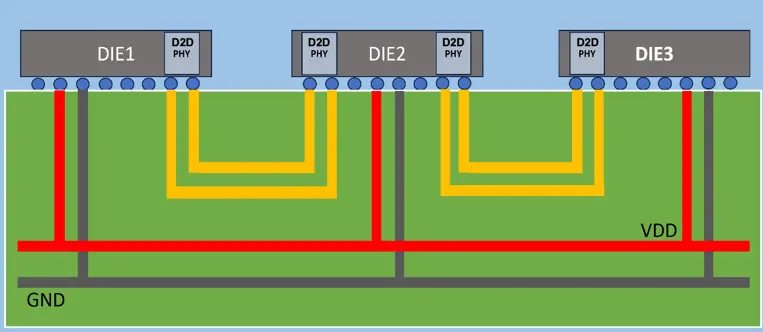
\includegraphics[width=0.6\textwidth]{img/2-1.png} % 图片文件名,不需要加扩展名
	\caption{简化的 Chiplet 标准封装视图 \cite{PiacentiniFilho2024Chiplet}}
	\label{fig:example}
\end{figure}

\subsection{Die 的应用场景}

传统的集成电路设计(如早期CPU、手机SoC)主要采用单Die芯片(Monolithic Die),将整个系统级芯片(SoC)的功能集中集成在一个晶粒上。
随着工艺发展,工业界转向了多Die系统(Multi-Die System),即在一个封装内通过先进封装技术互联多个独立制造的Die,这包括HBM内存堆叠和Chiplet架构。

在Chiplet架构中,Die分区的结果直接对应于Chiplet的划分:每个Chiplet就是一个功能独立制造的Die(芯片裸片),例如AMD CPU中的计算核心Die和I/O Die。
在Chiplet语境下,Die分区通常就是指Chiplet划分的结果——每个Chiplet就是一个独立的Die。

\begin{table}[htbp]
	\centering
	\caption{Chiplet划分与Die分区对比}
	\begin{tabular}{{c|c|c}}
		\hline
		 & Chiplet划分 & Die分区 \\
		\hline
		定义 & 功能/架构层面的模块拆分 & 物理实现层面的芯片分割 \\
		\hline
		层面 & 设计/架构层 & 物理/制造层 \\
		\hline
		目的 & 模块化、复用、异构集成 & 实现多芯片集成、提升良率 \\
		\hline
		关系 & Chiplet划分决定了Die分区的方式 & Die分区是Chiplet划分的物理实现 \\
		\hline
	\end{tabular}
\end{table}